\documentclass[a4paper,10pt]{report}
\usepackage[utf8]{inputenc}
\input{/home/andi/Studium/LaTex/preambel.tex}


%opening
\title{Magnetic Excitations In Iridiates}
\author{Andreas Karl Leonhardt}

\begin{document}

%\maketitle

%\begin{abstract}

%\end{abstract}
\tableofcontents

\chapter{Introduction}
\section{Towards A Spin Hamiltonian}

\subsection{Iridium And Compounds}
Iridium is a transition metal, i.e. it has a only partially filled $d$ shell.  
The shell structure of atomar Ir is given by $[\mathrm{Xe}]4f^{14}5d^7 6s^2$.
% ${\mathrm{Sr}}_{2}{\mathrm{IrO}}_{4}$
In the compounds treated in this thesis Iridium is oxidized to $\mathrm{Ir}^{4+}$ 
removing the $6s^2$ electrons as well as two electrons from the $5d$ shell. 
The ion has therefore $5d^5$ as the outermost and active shell ~\cite{Abragam70}.

%(the ion shell structure does not follow the Aufbau principle. 
%Therefore has $\mathrm{Ir}^{4+}$ a different shell structure than Tantalum, even though they have the same number of electrons. 
%This is because of the different charge of the nucleus, that leads to a greater seperation in energs levels with different quantum number n ($\propto \frac{Z}{n^2}$)).

The other elements of the compunds treated in this thesis have closed shells an are therefore spin free. In the case of $\mathrm{Ir}^{4+}$, 
$\mathrm{O}^{2-}$ has only closed shells ($1s^2,2s^2,2p^6$) and therefore is $L=S=0$.
the same holds for $\mathrm{Sr}^{2+}$ with the electron configuration of $\mathrm{Kr}$

\subsection{Ligand Field}

Embedded in the crystal of the compound, total rotational symmetry is broken and reduced to discrete symmetries about certain axes. 
This splits up the former degenerate $5d$ levels. 
In all of the compunds lookes at here, the $\mathrm{Ir}$ atoms are surrounded by octahedral of double negatively charged oxygen ions, the so called ligands. 
Those octahedra might share corners or even edges, while the latter one simply means they share two edges. 
%
% In ${\mathrm{Sr}}_{2}{\mathrm{IrO}}_{4}$ the $\mathrm{Ir}^{4+}$ is surrounded by 8 $\mathrm{O}^{2-}$, building a octaeder with shared corners.
%
The field generated by those ligands split up the $5d$ levels in the threefold $t_{2g}$ and the twofold $e_g$ states. 
Since the ligand field is quite strong
\todo{quote, strong compared to what, Hund's rule and why it is violated}
only the $t_{2g}$ levels are populated in the ground state, leaving one hole in this band. 
The $e_g$ orbitals are not occupied in the ground state, since the crystal field splitting is stronger than the repulsion of electrons beeing in the same orbital. 
This leads to the so calles low-spin state, in contrast to a weak crystal field, 
where it would be more favourable to follow Hund's rules, 
i.e. filling up the $t_{2g}$ and the $e_g$ orbitals with electrons of the same spin, before putting to electrons with opposite spin into an orbital.
The $t_{2g}$ levels build an \emph{effective} $L=1$ system, since it is threefold degenerate.

\subsection{Strong Spin-Orbit Coupling}

In the $5d$ elements spin orbit coupling (SOC) plays an important role since it increases with the charge of the nucleus.
\todo{theoretical background for string SOC according to Z.}
Since there is one hole in the $t_{2g}$ shell left, the total Spin is $S=\frac12$. 
When coupled to the effective spin $L=1$ as mentioned above, 
the sixfold degenerate $t_{2g}$ states (including spin degeneracy) split into a fourfold degenereate level with $J=\frac32$
and twofold degenerate level with $J=\frac12$. The latter one is higher in energy, since we couple an \emph{effective} angular momentum to the spin,
thus the paralell coupling is energetically favourable.
In the ground state the $J=\frac32$ band will be filled, while the $J=\frac12$ band is half filled, leaving us with an effective Spin$\frac12$ system on each Iridium site in the grid.
\todo{create/include graph similar to \cite{PhysRevLett.101.076402}}

The two states are given by a linear combination of the molecular orbits and spin states,
\begin{equation}
 \ket{J_{\mathrm{eff}} =\frac12, M_{J_{\mathrm{eff}}}= \pm \frac12}
 = 
 \frac{1}{\sqrt{3}} \left( \ket{yz,\pm \sigma} \mp \im \ket{zx,\pm \sigma} \mp \ket{xy,\mp \sigma} \right).
\end{equation}
where $+\sigma = \uparrow, -\sigma = \downarrow$. The moelcular orbits are given by linear combinations of the spherical harmonics
\begin{IEEEeqnarray}{rCl}
\ket{xz} &=& \frac{1}{\sqrt{2}} \left( Y_2^{-1} - Y_2^{1} \right) \\
\ket{yz} &=& \frac{\im}{\sqrt{2}} \left( Y_2^{-1} + Y_2^{1} \right) \\
\ket{xy} &=& \frac{\im}{\sqrt{2}} \left( Y_2^{-2} - Y_2^{2} \right) 
\end{IEEEeqnarray}

\todo{transformation properties of the ground state}


\subsection{Spin System And The Hubbard Model}

\subsubsection{Tight Binding Model} % in second quantization




Energy eigenstates of the crystal must be Bloch states, defined by  the relation
\begin{equation}
 \Psi_{n,\vec{k}} \left( \vec{r}+\vec{t}\right) = \euler^{\im \vec{t} \vec{k} } u_{n,\vec{k}} \left( \vec{r} \right), \label{BlochDef}
\end{equation}
where $\vec{t}$ denotes a translation vector of the lattice, e.g. one that leaves the lattice unchanged, 
and $u_{n,\vec{k}}$ is a periodic function with the same periodicity than the lattice.
Using a Fourier transform on the Bloch states of different bands $n$, we get the so called Wannier states,
\begin{equation}
 \Psi_{\vec{R}_i, n} \left( \vec{r} \right) = \frac1{\sqrt{N}} \sum_{\vec{k}} \euler^{\im \vec{k}\vec{R}_i } \Psi_{\vec{k}, n} 
\end{equation}
Those are no longer eigenstates of the Hamiltonian, but still orthonormal, since the transformation is unitarian. 
Furthermore they are localized around the positions $\vec{R}_i$.
Instead of the eigenfunctions of the single particle Hamiltonian, we can use linear combinations of them. 
This gives us a different set of Wannier functions, that are related to the ones previously defined by another unitary transformation.
The additional degrees of freedom can be used to optimize the Wannier functions according to certain criteria.
The most common ones are maximal localization or symmetries of the crystal or the atomic orbitals.



For atoms with a very large distance in between them the Wannier functions approach states of free atoms or linear combinations of them.
Each band corresponds to a atomic orbital or a set set of degenerate orbitals.
If the overlap of the potentials of the atoms building up the crystal is small, we might use atomic states as a starting point for our description of the system.
We can construct a Bloch function by
\begin{equation}
 \Psi_k(\vec{r}) = \sum_{\vec{R}} \euler^{\im \vec{k}\vec{R} }  \phi_{n}(\vec{r}-\vec{R}). 
\end{equation}
This construction fullfills the requirement of \ref{BlochDef}, since
\begin{equation}
 \Psi_{n,k}(\vec{r}+\vec{t}) 
 = \euler^{\im \vec{k} \vec{t} } \sum_{\vec{R}} \euler^{\im \vec{k} (\vec{R}-\vec{t})} \phi_n (\vec{r}-\vec{R}+\vec{t}) 
 = \euler^{-\im \vec{k} \vec{t} } \sum_{\vec{R}} \euler^{\im \vec{k}\vec{R} }  \phi_{n}(\vec{r}-\vec{R}), 
\end{equation}
where the second step is due to invariance under a translation of the lattice $\vec{t}$.
The Bloch functions constructed in this way are in general not orthogonal.
By taking a relevant subset of atomic states, and defining for each $\vec{k}$
\begin{equation}
 H_{nm} = \bra{\Psi_{n,\vec{k}}} H \ket{\Psi_{m,\vec{k}}} \text{  and  } S_{nm} = \braket{\Psi_{n,\vec{k}}}{\Psi_{m,\vec{k}}}
\end{equation}
we can set up the secular equation
\begin{equation}
 \det(H_{nm}-E_kS_{nm})=0.
\end{equation}
This gives us the band energies. The corresponding eigenstates are called Löwedin functions.
% BAD writing here, tsss. What is the poinit anyway?
% resemble the Löwedin states the crystal symmetry? They should (--> see Slater et al.)



In this picture we think of electrons as being in a certain state of an atom and hopping to other states rather then being delocalized over the whole crystal.
In any real system the states will have some overlap, creating the possibility for electrons to hop between different sites.

Using second quantization, we can make the above transformation for creation and annihilation operators as well.
The relation between creation and annihilation operators for Bloch states and Wannier states is then given by
\begin{IEEEeqnarray}{rCl}
  a^{\dagger}_{i , n}  =  \sum_{\vec{k}} \euler^{\im \vec{k}\vec{R}_i } a^{\dagger}_{\vec{k} , n}, 
      &\quad&
  a_{i , n}  =  \sum_{\vec{k}} \euler^{-\im \vec{k}\vec{R}_i } a_{\vec{k} , n},  \nonumber\\  
  a^{\dagger}_{\vec{k} , n}  =  \sum_{i} \euler^{-\im \vec{k}\vec{R}_i } a^{\dagger}_{i , n}
    &\quad&
  a_{\vec{k} , n}  =  \sum_{i} \euler^{\im \vec{k}\vec{R}_i } a_{i , n}.
\end{IEEEeqnarray}
By construction they fullfill the anticommutation relations for fermion creation and annihilation operators. 
The correlation is taken into account by introducing a two particle operator. 
Since the single particel Hamiltonian $H_0$ is diagonal for the Bloch states, we can write
\begin{IEEEeqnarray}{rCl}
 H_0 &=& \sum_{\vec{k}} E_{\vec{k}} a^{\dagger}_{\vec{k}} a_{\vec{k}} \nonumber \\
    &=& \sum_{ij} \underbrace{ \frac1N \sum_{\vec{k}} E_{\vec{k}} \euler^{\im \vec{k} ( \vec{R}_i -\vec{R}_j ) } }_{t_{ij}} a^{\dagger}_{i} a_{j},
\end{IEEEeqnarray}
defining the one particle operator $t_{ij}$. 
The diagonal terms $t_{ii}$ are the single particle energys of the atomic sites, 
while the off-diagonal elements provide the hopping.
In cases where the tight binding is a good approximation those hopping elements will fall off quite fast and 
we might include only interactions between close neighbours, usually between nearest neighbours and maybe next-to-nearest neighbours.
So far we did not take electron-electron interactions into account. 
This can be done by introducing the two particle operator
\begin{equation}
 H_{\text{int}} = \sum_{ijkl} U_{ijkl} a^{\dagger}_i a^{\dagger}_j a_k a_l
\end{equation}
where the matrix elements $U_{ijkl}$ are given by
\begin{equation}
 U_{ijkl} = \int \!  \dint^3 r \, \dint^3 r^{\prime} \,  \Psi_i^*(\vec{r}) \Psi_j^*(\vec{r}^{\prime}) V(\vec{r}-\vec{r}^{\prime} ) \Psi_k(\vec{r}) \Psi_l(\vec{r}) 
\end{equation}
Due to the small overlap of different states, usually only a few matrix elements are of relevant magnitude, a long range interaction is however possible.
The diagonal matrix elements $U_{iii} = U$ account for the repulsion between electrons on the same site and are certainly the most important contribution.
Because of the Pauli principle they have to have opposite spins. 
This is guaranteed by the anticommutation relation of creation and annihilation operators.
Including spin notation in the creation and annihilation operators, we can simplify the interaction contribution to 
\begin{equation}
 H_{\text{int}} = U \sum_i n_{i,\uparrow} n_{i,\downarrow},
\end{equation}
using the number operator $n_{i,\sigma} = a^{\dagger}_{i,\sigma} a_{i,\sigma}$.
This is the only term taken into account for the Hubbard model.
However, reducing an interaction that is not necessarily local to only on-site interactions is a grave simplification, 
neglecting the vast amount of parameters in the interaction matrix $U_{ijkl}$ and therefore long range repulsion.
The interaction seems to be lower than what you would expect from an correlation integral of the corresponding orbitals.
\todo{only when supportable with citation. Article about Hubbard in general?}
It is not possible to link the parameter $U$ to a physical quantity directly
and the Hubbard model is therefore not a first principle model. $U$ has to be seen as an effective parameter, that has to be adjusted according to experiments or calculations using
other methods.
The single particle part of the Hamiltonian however can be taken from first principle methods such as density funcitonal calculations\todo{DFT here?}.


% other interactions 
% U_{ijji}, Heisenberg
% U_{iijj}, density fluctuations

% superexchange?










\subsubsection{Relative Orientation Of Octahedra}

% rotation by 11° in Sr$_2$IrO$_4$, corner sharing
% edge sharing in other materials, non 2D setup



To describe the above spin system there are several models. We assumed the tight binding approximation to be valid, i.e. atomic orbitals
are still a good description for electrons and they are localized. However, their wavefunctions have a certain overlap and there is a correlation. 
%In the Heisenberg model this correlation is not taken into account, the Hamiltonian describes only spin interaction. 
%\begin{equation}
% \hat{H} =  -J \sum_{<i,j>} \hat{\mathbf{S}}_i\hat{\mathbf{S}}_j
%\end{equation}
%where $<i,j>$ indicates a sum over nearest neighbours and the spin operator is $\hat{\mathbf{S}}_i = \frac12 \left( \sigma^x_i, \sigma^y_i, \sigma^z_i \right)^{\intercal}$.
%The model can be extended to next-to-nearest neighbour interactions and so on. 

\section{to be redone}

However, since electrons with opposite spin can occupy the same state and repell each other, this might have to be taken into account, depending on the 
strength of the correlation in such a situation. 
This can be done in the Hubbard model, given by
\begin{equation}
 \hat{H} = \underbrace{U \sum_i c^{\dagger}_{i,\uparrow}c_{i,\uparrow} c^{\dagger}_{i,\downarrow}c_{i,\downarrow} }_{\text{correlation}}
	    -\underbrace{t \sum_{<i,j>,\sigma} c^{\dagger}_{i,\sigma}c_{j,\sigma} + c^{\dagger}_{j,\sigma}c_{i,\sigma} }_{\text{hopping term}}
\end{equation}
with the creation operator 
\begin{equation}
 c^{\dagger}_{i} = \euler^{-\im\pi \sum_{j<i} a^{\dagger}_j a_j } a^{\dagger}_i\quad ; \quad a^{\dagger}_i = \frac12 \left( \sigma^x_i + \im \sigma^y \right)
\end{equation}
and the corresponding annihilation operator. 
 this kind of creation operator phase correction is only needed when derived from the Heisenberg model, see Quantum Many Particle Systems by Negele
In certain situations the Heisenberg model can be derived from the Hubbard model. 

\section{Band Structure}

% Insulator (band splitup using U)
% How U changes the picture

\subsection{Momentum Space}

The Hubbard model is defined by the Hamiltonian
\begin{equation}
 \hat{H} = \hat{H}_0
	   + U \sum_i c^{\dagger}_{i,\uparrow}c_{i,\uparrow} c^{\dagger}_{i,\downarrow}c_{i,\downarrow} 
	    . \label{Hubbard_space}
\end{equation}
with a band structure single particle Hamiltonian $\hat{H}_0$.


In the simplemost version only nearest neighbour hoppings are taken into account,
\begin{equation}
 \hat{H}_0 = - t \sum_{\langle i,j \rangle,\sigma} \left (c^{\dagger}_{i,\sigma}c_{j,\sigma} + c^{\dagger}_{j,\sigma}c_{i,\sigma} \right) 	    -\mu \sum_{i,\sigma} c^{\dagger}_{i,\sigma}c_{i;\sigma}
\end{equation}
where $\langle i,j \rangle$ denotes a sum over pairs of nearest neighbours, counting each pair only once.
The first term in $\hat{H}_0$represents the kinetic energy of particles, hopping from one site to a neighbouring site.
The chemical potential is represented in the second term, showing the energetic cost to add a particle to the system.
As an external parameter it can be used to control the particle density $n$, that is the number of particles per site.
% \mu = \frac{U}{2} is explained later, when dealing with half filling in greater detail


In order to represent the Hamiltonian in momentum space we use the relation between the representation of creation and annihilation operators in real space and momentum space,
\begin{equation}
 c^{\dagger}_i=N^{-\frac12} \sum_k \euler^{-\im \vec{k}\vec{R}_i } c^{\dagger}_k, \qquad c_i= N^{-\frac12} \sum_k \euler^{\im \vec{k}\vec{R}_i } c_k.
\end{equation}
Inserting this relation and using 
\mbox{$\sum_i \euler^{(\vec{k}-\vec{l})\vec{R}_i } = N\delta_{\vec{k}\vec{l}}$} 
the chemical potential term translates to
\begin{equation}
 -\mu \sum_{i,\sigma} c^{\dagger}_{i,\sigma}c_{i;\sigma} = 	-\mu \sum_{\vec{k},\sigma} c^{\dagger}_{\vec{k},\sigma}c_{\vec{k}\sigma}
\end{equation}
In a similar manner the first term in $\hat{H}_0$ turns into	
\begin{IEEEeqnarray}{c}
 -\frac{t}{N} \sum_{\vec k \vec l ,\sigma} \sum_{<i,j>} 
	      \left( 
	      \euler^{-\im \left(  \vec{k}\vec{R}_i - \vec{l}\vec{R}_j\right)} c^{\dagger}_{\vec{k},\sigma} c_{\vec l, \sigma}  
	      + \euler^{-\im \left(  \vec{k}\vec{R}_j - \vec{l}\vec{R}_i \right)} c^{\dagger}_{\vec{k},\sigma} c_{\vec l, \sigma} 
	      \right)	      
	      \label{ham_pspace}
\end{IEEEeqnarray}
We can now reparametrize the sum over nearest neighbours, using the translation vectors $\vec{T}_d$ between nearest neighbours,
\begin{equation}
 \sum_{\langle i,j \rangle} = \sum_i \sum_d \quad; \quad \vec{R}_j = \vec{R}_i + \vec{T}_d
\end{equation}

We can therefore write \ref{ham_pspace} as
\begin{IEEEeqnarray}{Cl}
 & -\frac{t}{N} \sum_{\vec{k},\vec{l},\sigma} \sum_{i} \euler^{-\im \left(\vec{k}-\vec{l} \right)\vec{R}_i } 
    \sum_d \left(\euler^{-\im \vec{k}\vec{T}_d} + \euler^{\im  \vec{l} \vec{T}_d} \right) 
    c^{\dagger}_{\vec{k},\sigma}c_{\vec{l},\sigma} \nonumber \\
    =& \sum_{\vec{k},\sigma}  c^{\dagger}_{\vec{k},\sigma}c_{\vec{k},\sigma}  \underbrace{\sum_d -2t \cos( \vec{k} \vec{T}_d ) }_{\varepsilon_{\vec k} }
\end{IEEEeqnarray}
which shows that the single-particle Hamiltonian  is  diagonal in momentum space.

In the case of a two dimensional square lattice, the translational vectors of nearest neighbours are given by the lattice constant $a$ times the unit vectors in 
$x$- and $y$-direction, $T_d = a\cdot \vec{e}_d$, $ d \in \{x,y\}$ as shown in figure \ref{2d_square}.
Using $a$ as the basic length unit, that is $a=1$, 
and normalizing therefore the momentum to the intervall $[-\pi,\pi]\times [-\pi,\pi]$ 
we get in this case
$\varepsilon_{\vec k} = \mbox{$-2t\cos(k_x)-2t\cos(k_y)$}$. 

\begin{figure}
\begin{center}
 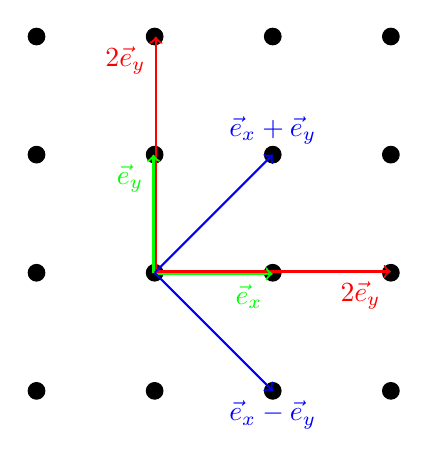
\begin{tikzpicture}[scale=1.5]
 \foreach \x in {1,...,4}
 \foreach \y in {1,...,4}
 \filldraw  (\x,\y) circle (2pt);
 \draw[->,red  ,thick] (2.01,2) -- (2.01,4) node[anchor=north east] {$2\vec e_y$};
 \draw[->,red  ,thick] (2,2.01) -- (4,2.01) node[anchor=north east] {$2\vec e_y$};
 \draw[->,green,thick] (1.99,2) -- (1.99,3) node[anchor=north east] {$\vec e_y$};
 \draw[->,green,thick] (2,1.99) -- (3,1.99) node[anchor=north east] {$\vec e_x$};
 \draw[->,blue ,thick] (2,2) -- (3,3) node[anchor= south] {$\vec e_x+ \vec e_y$};
 \draw[->,blue ,thick] (2,2) -- (3,1) node[anchor=north ] {$\vec e_x- \vec e_y$}; 
 \end{tikzpicture}
\end{center}
\caption{translation vectors $\vec T_d$ in a two dimensional square grid with first (green), second (blue) and third (red) neighbour interactions}
\label{2d_square}
\end{figure}

In an more elaborate approach we might add second and third neighbour hoppings. 
They can be treated in the same manner as nearest neighbours, simply by including the corresponding vectors $\vec T_d$ with their respective couplings.
The vectors up to third neighbour interactions are shown in figure \ref{2d_square}. 
We extend the single-particle Hamiltonian in real space to
\begin{IEEEeqnarray}{rCl}
 \hat{H}_0 &=& 
 - t \sum_{\langle i,j \rangle,\sigma} \left( c^{\dagger}_{i,\sigma}c_{j,\sigma} + c^{\dagger}_{j,\sigma}c_{i,\sigma} \right)
 - t^{\prime} \sum_{\langle \langle i,j \rangle \rangle ,\sigma} \left( c^{\dagger}_{i,\sigma}c_{j,\sigma} +c^{\dagger}_{j,\sigma}c_{i,\sigma} \right) \nonumber \\ &&
 - t^{\prime \prime} \sum_{\langle \langle \langle i,j \rangle \rangle \rangle ,\sigma} \left( c^{\dagger}_{i,\sigma}c_{j,\sigma}   + c^{\dagger}_{j,\sigma}c_{i,\sigma} \right)
 -\mu \sum_{i,\sigma} c^{\dagger}_{i,\sigma}c_{i;\sigma}
\end{IEEEeqnarray}
Double and triple brackets denote second- and third-neighbour pairs respectively and again, the sum counts each pair only once.
The resulting expression for the energy dispersion reads
\begin{equation}
 \varepsilon_{\vec k } = -2t \left(\cos k_x + \cos k_y \right) -4t^{\prime} \cos k_x \cos k_y  -2t^{\prime \prime} \left( \cos 2k_x + \cos 2k_y \right)
\end{equation}




The interaction term translates to
\begin{IEEEeqnarray}{rl}
 &\frac{U}{N^2} \sum_{\vec{k}\vec{l}\vec{m}\vec{n}} \sum_i \euler^{-\im (\vec{k}-\vec{l}+\vec{m}-\vec{n})\vec{R}_i } 
    c^{\dagger}_{\vec{k},\uparrow}c_{\vec{l},\uparrow} c^{\dagger}_{\vec{m},\downarrow}c_{\vec{n},\downarrow} \nonumber \\
    =& \frac{U}{N} \sum_{\vec{k}\vec{l}\vec{m}\vec{n}} \delta(\vec{k}-\vec{l}+\vec{m}-\vec{n} )
	c^{\dagger}_{\vec{k},\uparrow}c_{\vec{l},\uparrow} c^{\dagger}_{\vec{m},\downarrow}c_{\vec{n},\downarrow} \nonumber \\
    =& \frac{U}{N} \sum_{\vec{k}\vec{k}^{\prime}\vec{q}}
	c^{\dagger}_{\vec{k},\uparrow}c_{\vec{k}-\vec{q},\uparrow} c^{\dagger}_{\vec{k}^{\prime},\downarrow}c_{\vec{k}^{\prime}+\vec{q},\downarrow}
 \end{IEEEeqnarray}
where we choose a convenient parametrization for the sum over the momenta in the last line.
This term is non-diagonal, but it ensures momentum conversation at each vertex.

The total expression for the Hamiltonian in momentum space reads
 \begin{equation}
  \hat{H} = \sum_{\vec{k},\sigma} \left(\varepsilon_{\vec k} - \mu\right) c^{\dagger}_{\vec{k},\sigma}c_{\vec{k}\sigma} + \frac{U}{N} \sum_{\vec{k}\vec{k}^{\prime}\vec{q}}
	c^{\dagger}_{\vec{k},\uparrow}c_{\vec{k}-\vec{q},\uparrow} c^{\dagger}_{\vec{k}^{\prime},\downarrow}c_{\vec{k}^{\prime}+\vec{q},\downarrow}
 \end{equation} 

\section{Mean Field Equations}

\subsubsection{The Mean-Field Hamiltonian}

We treat the Hubbard model in a pertubative approach at the mean-field level.
The Hubbard term  $H_U$ acts as the pertubation.
As a two-particle operator it can be read as a product of two single particle opearators.
We can rewrite any product of two operators $\hat{A}$ and $\hat{B}$ as
\begin{IEEEeqnarray}{rCl}
 \hat{A}\cdot\hat{B} 
		    &=&	 \left(\hat A - \langle \hat A \rangle \right) \left( \hat B -\langle \hat B \rangle \right)
			 +\langle \hat A \rangle \hat B
			 +\langle \hat B \rangle \hat A
			 - \langle \hat A \rangle \langle \hat B \rangle
\end{IEEEeqnarray}
In the mean field approach we neglect the first term on the right hand side –the product of fluctuations around their expectation value– leaving us with
\begin{equation}
  \hat{A}\cdot\hat{B} 
		   \approx 
			 \langle \hat A \rangle \hat B
			 +\langle \hat B \rangle \hat A 
			 - \langle \hat A \rangle \langle \hat B \rangle
\end{equation}
% RPA has nothing to do with this I think…
%
We use this relation on the single particle oparators 
$c^{\dagger}_{\vec k,\uparrow}c_{\vec k - \vec q,\uparrow}$
and 
$c^{\dagger}_{\vec k,\downarrow}c_{\vec k + \vec q,\downarrow}$
in the Hubbard term of the Hamiltonian. 
Furthermore, we drop the constant term corresponding to $\langle \hat A \rangle \langle \hat B \rangle$, since a constant in the Hamiltonian will not have any
influence on the dynamic of the system. 
The mean-field approxiamtion of the Hubbard term reads
\begin{equation}
 H_U \stackrel{\mathrm{mf}}{\approx}  \frac{U}{N}
 \sum_{\vec{q}} \sum_{\sigma} 
 \left( \sum_{\vec{p}^{\prime}} \langle c^{\dagger}_{\vec{p}^{\prime},-\sigma} c_{\vec{p}^{\prime}+\vec{q},-\sigma} \rangle \right)
	\sum_{\vec p}  c^{\dagger}_{\vec{p},\sigma} c_{\vec{p}-\vec{q},\sigma}. \label{Hubbard_mean_field}
\end{equation}
The expectation value for the one particle operator is different from zero for only two values of $\vec q$.
First, for $\vec q = 0$ we get the number density of particles with the corresponding spin $\sigma$,
\begin{equation}
 n_{\sigma} = \frac1N \sum_{\vec k} \langle c^{\dagger}_{\vec k, \sigma} c_{\vec k, \sigma} \rangle.
\end{equation}


% elaborat on the meaning of n_\sigma here, bzw. at half filling osv.

%
%
% meaning of mean-field
%
% symmetry bracking, antiferromagnetic ground state
%
%propagators: diagonal, offdiagonal
%
% validity range of the above assumptions: symmetrie, metal insulator transition; limits and corrections
%
%RPA
%
%
The second contribution comes from $\vec q = (\frac12, \frac12)$.
This vector acts as a nesting vector for the Fermi surface of the band structure. 
A square lattice with only nearest-neighbour interactions can be divided into two sublattices. 
Hoppings occur only from one sublattice to the other and as a result we get a perfectly nested energy dispersion,
that is
$\varepsilon_{\vec k} = -\varepsilon_{\vec k + \vec Q}$ with the nesting vector $\vec Q = (\frac12,\frac12)$.
The Fermi surface in this case is therefore a perfect square. 
Introducing higher order hopping terms deforms it, but nesting with $\vec Q$ holds on a approximate level for small $t^{\prime}$ and $t^{\prime \prime}$.
The Fermi surfaces with nesting vector $\vec Q$ for two different sets of parameters are shown in \ref{fig:energie_dispersion}.
%
%
\begin{figure} \centering
\begin{subfigure}{0.49\linewidth} \centering
 \includegraphics[width=\textwidth]{../bandstructure_t.pdf}
 \caption{$ t^{\prime}=t^{\prime \prime} =0$ }
 \label{fig:dispt}
\end{subfigure}
\begin{subfigure}{0.49\linewidth}
  \includegraphics[width=\textwidth]{../bandstructure_ttt.pdf}
  \caption{ $t^{\prime}= 0.2326t$, $t^{\prime \prime} = 0.1163t$}
  \label{fig:dispttt}
\end{subfigure}
\caption{single particle energy dispersion in units of t, momenta in units of $2\pi$. Shows the nesting vector }
\label{fig:energie_dispersion}
\end{figure}
%
%$\vec Q$ is the basis vector for antiferromagnetic ordering. 
%This is observed in these materials \todo{how general, which ones} and expected % for what reason?
Nesting with $\vec Q = (\frac 12, \frac12)$ leads to a symmetrie broken ground state with an antiferromagnetic moment. 
\todo{why do we expect SB? How does this arise from a nested Fermi surface?}. 
The expectation value of the staggered magnetization, given by
\begin{IEEEeqnarray}{lCl}
 m_{s} &=& m_{s, \uparrow} - m_{s, \downarrow}, \\
 m_{s, \sigma} &=& \frac1N \sum_{\vec k} \langle c^{\dagger}_{\vec k , \sigma} c_{\vec k + \vec Q, \sigma} \rangle,
\end{IEEEeqnarray}
is therefore non-zero. 

In terms of the above defined parameters equation \ref{Hubbard_mean_field} simplifies finally to
\begin{equation}
 \hat H = \sum_{\vec k, \sigma} \left( \varepsilon_{\vec k } - \mu + U n_{-\sigma} \right) c^{\dagger}_{\vec k, \sigma} c_{\vec k ,\sigma}
	  + U m_{s,-\sigma} \sum_{\vec k, \sigma} c^{\dagger}_{\vec k + \vec Q, \sigma} c_{\vec k, \sigma}.
\end{equation}
%
%\begin{equation}
% H_U \approx \sum_{\sigma} \left( U n_{-\sigma} \sum_{\vec{p}} c^{\dagger}_{\vec{p}, \sigma} c_{\vec p, \sigma} 
%	      + \frac{ U m_{s,-\sigma}}2
%			      \sum_{\vec p} \left(  c^{\dagger}_{\vec{p}+\vec Q, \sigma} c_{\vec p, \sigma} 
%	                                          + c^{\dagger}_{\vec{p}       , \sigma} c_{\vec p+ \vec Q, \sigma} \right) \right)
%\end{equation}
%
%\begin{IEEEeqnarray}{rCl}
% H_{\mathrm{mf}} &=
%		\sum_{\vec{p},\sigma} &
%				      \left( \varepsilon_k - \mu + U n_{-\sigma} \right) 
%					  c^{\dagger}_{\vec{p},\sigma} c_{\vec{p},\sigma}
%				      +\frac{U}2  m_{s,-\sigma}	 
%					  \left( c^{\dagger}_{\vec{p}+\vec{Q},\sigma} c_{\vec{p},\sigma} +\mathrm{h.c.} %c^{\dagger}_{\vec{p},\sigma} c_{\vec{p}+\vec{Q},\sigma} 
%					  \right)					 
%\end{IEEEeqnarray}
%
One can clearly see the mean repulsion proportional to the number density of particles with opposite spin due to the nature of the interaction,
as well as the staggered field from the ground state. 

\subsubsection{Mean-Field Propagators}

The mean-field Hamiltonian gives rise to two different propagators.
First we get the diagonal contribution, second an off-diagonal one from the staggered component. 
The propagators are defined by
\begin{IEEEeqnarray}{rCl}
 G_{\vec k}(\tau) &=& -\langle \mathcal{T}_{\tau} c_{\vec k         ,\sigma}(\tau)  c^{\dagger}_{\vec k ,\sigma}(0) \rangle \\
 F_{\vec k}(\tau) &=& -\langle \mathcal{T}_{\tau} c_{\vec k +\vec{Q},\sigma}(\tau)  c^{\dagger}_{\vec k ,\sigma}(0) \rangle \\ \label{Def_Propagator}
\end{IEEEeqnarray}
with the imaginary time ordering operator $\mathcal{T}_{\tau}$, acting on a pair of fermion operators according to
\begin{IEEEeqnarray}{rCl}
 \mathcal{T}_{\tau} \hat{A}(\tau_1) \hat{B}(\tau_2) &=&
 -\Theta(\tau_1-\tau_2)\hat{A}(\tau_1) \hat{B}(\tau_2) + \Theta(\tau_2-\tau_1)\hat{B}(\tau_2) \hat{A}(\tau_1) \nonumber \\
 &=& \left\{ \begin{array}{r@{\text{ for }}l} -\hat{A}(\tau_1) \hat{B}(\tau_2) & \tau_1 \ge \tau_2 \\ \hat{B}(\tau_2) \hat{A}(\tau_1) & \tau_1 < \tau_2 \end{array} \right.
\end{IEEEeqnarray}
For the behaviour at $\tau=0$ as shown in the last line, we need the convetion of $\Theta(0)=\frac12$.
From this definition follows that $n_\sigma$ and $m_{s,\sigma}$ can be expressed in terms of propagators, namely through
\begin{IEEEeqnarray}{lCl}
 n_{\sigma} &=& \frac1N \sum_{\vec k} \left( 1-G_{\vec k, -\sigma}(0) \right) \label{n_DEF}\\
 m_{s,\sigma} &=& -\frac1N \sum_{\vec k} F_{\vec k, -\sigma}(0)		\label{m_DEF}
\end{IEEEeqnarray}


From the definition of the propagtors in \ref{Def_Propagator} and the equation of motion for operators, 
$\frac{\dint}{\dint \tau} \hat{A} = [H,\hat{A}] + \frac{\partial}{\partial_{\tau}} \hat{A}$,
we get the differential equation
\begin{IEEEeqnarray}{rCl}
 \partial_{\tau} G_{\vec k ,\sigma}(\tau) 
 &=&
 \delta(\tau) \langle c_{\vec k ,\sigma}(\tau) c^{\dagger}_{\vec k ,\sigma}(0) + c^{\dagger}_{\vec k ,\sigma}(0) c_{\vec k ,\sigma}(\tau) \rangle \nonumber \\&&
 + \Theta(\tau) \langle [\hat H , c_{\vec k ,\sigma}(\tau)] c^{\dagger}_{ \vec k ,\sigma}(0) \rangle		\nonumber \\ &&
 -  \Theta(-\tau) \langle c^{\dagger}_{ \vec k ,\sigma}(0) [\hat H , c_{\vec k ,\sigma}(\tau)]  \rangle \label{EOM_G}
\end{IEEEeqnarray}
Here we used $\partial_{\tau} \Theta(\tau) = \delta(\tau)$.
The commutators can be evaluated using the identity $[AB,C] = A\{B,C\} - \{A,C\}B$ and the anticommutation rules for the creation and annihilation operators.
\todo{give fermion commutation rules somewhere earlier}
This leaves us with
\begin{equation}
 [H,c_{\vec k ,\sigma}(\tau)]=-\left(\varepsilon_{\vec k}-\mu + Un_{-\sigma} \right) c_{\vec k ,\sigma}(\tau) - Um_{s,-\sigma} c_{\vec k +\vec{Q},\sigma}(\tau)
\end{equation}
Putting this back in \ref{EOM_G} together with the definitions for $G$ and $F$, we get
\begin{IEEEeqnarray}{rCl}
  \partial_{\tau} G_{\vec k ,\sigma}(\tau) 
&=&
\delta(\tau)\langle \{c_{\vec k ,\sigma}(\tau),c^{\dagger}_{\vec k ,\sigma}(0)\} \rangle
- \left( \varepsilon_{\vec k }-\mu+ Un_{-\sigma} \right) G_{\vec k ,\sigma}(\tau)  \nonumber \\ &&
 -Um_{s,-\sigma} F_{\vec k ,\sigma}(\tau) \label{EOM_G_II}
\end{IEEEeqnarray}
In a next step we want to take the Fourier transform of this equation. 
The Fourier transformed propagator is related to the propagator in imaginary time through
\begin{IEEEeqnarray}{rCl}
 G_{\vec k ,\sigma}(\tau) &=& \frac{1}{\beta} \sum_n \euler^{-\im \omega_n \tau} G_{\vec k ,\sigma}(\im \omega_n) \\
 G_{\vec k ,\sigma}(\im \omega_n) &=& \int_0^{\beta} \! \!\dint  \tau \: \euler^{\im \omega_n \tau} G_{\vec k ,\sigma}(\tau)
\end{IEEEeqnarray}
The so called Matsubara frequencies $\omega_n$ are given by $\omega_n = \frac{\pi}{\beta}(2n+1), \; n \! \in \! \mathbb{Z}$.
This ensures the anti-periodicity of fermionic Greensfunctions, $G(\tau+\beta) = -G(\tau)$.
Transforming equation \ref{EOM_G_II} to momentum space we get
\begin{IEEEeqnarray}{rCl}
 \left( \im \omega_n -\varepsilon_{\vec k } +\mu - Un_{-\sigma} \right) G_{\vec k ,\sigma}(\im \omega_n) = 1 +Um_{s,-\sigma} F_{\vec k ,\sigma}(\im \omega_n)
\end{IEEEeqnarray}
In the same way, starting from $\frac{\dint}{\dint \tau} F_{\vec k ,\sigma}(\tau)$ we get for the off-diagonal propagator
\begin{IEEEeqnarray}{rCl}
 \left( \im \omega_n -\varepsilon_{\vec k +\vec{Q}} +\mu - Un_{-\sigma} \right) F_{\vec k ,\sigma}(\im \omega_n) = Um_{s,-\sigma} G_{\vec k ,\sigma}(\im \omega_n)
\end{IEEEeqnarray}
There is no constant term, since the anticommutator in \ref{EOM_G_II} is zero for off-diagonal momenta. 
Putting the last two equations together we get the expressions for the propagators
\begin{IEEEeqnarray}{rCl}
 G_{\vec k ,\sigma}(\im \omega_n) &=& \frac{ ( \im \omega_n - \varepsilon_{\vec k +\vec{Q}} + \mu -Un_{-\sigma} )}
			      { ( \im \omega_n - \varepsilon_{\vec k +\vec{Q}} + \mu -Un_{-\sigma} )
			        ( \im \omega_n - \varepsilon_{\vec k }         + \mu -Un_{-\sigma} )
			      - U^2m_{s,-\sigma}^2 } \nonumber \\
 F_{\vec k ,\sigma}(\im \omega_n) &=& \frac{ Um_{s,-\sigma}}
			    { ( \im \omega_n - \varepsilon_{\vec k +\vec{Q}} + \mu -Un_{-\sigma} )
			      ( \im \omega_n - \varepsilon_{\vec k }         + \mu -Un_{-\sigma} )
			      - U^2m_{s,-\sigma}^2 }			      
\end{IEEEeqnarray}
We can rewrite this in a more appealing way by factorizing the denominator of both propagators. 
The poles are located at
\begin{equation}
 E_{\vec k ,\sigma}^{\pm}
 =
 \frac{\varepsilon_{\vec k }+\varepsilon_{\vec k +\vec{Q}}}2 -\mu + Un_{-\sigma}  \pm \sqrt{ \left(\frac{\varepsilon_{\vec k }-\varepsilon_{\vec k +\vec{Q}}}2\right)^2 + U^2m_{s,-\sigma}^2 }
\end{equation}
Note that $E_{\vec k ,\sigma}^{\pm}=E_{\vec k +\vec{Q},\sigma}^{\pm}$, since $\varepsilon_{\vec k +2\vec{Q}}=\varepsilon_{\vec k }$.
With this, we can write the propagators as
\begin{IEEEeqnarray}{rCl}
 G_{\vec k ,\sigma}(\im \omega_n) &=& \frac{ \im \omega_n - \varepsilon_{\vec k +\vec{Q}} +\mu -Un_{-\sigma} }
					    { (\im \omega_n - E_{\vec k ,\sigma}^+) (\im \omega_n - E_{\vec k ,\sigma}^-) }
\\
 F_{\vec k ,\sigma}(\im \omega_n) &=& \frac{ Um_{s,-\sigma} }
					    { (\im \omega_n - E_{\vec k ,\sigma}^+) (\im \omega_n - E_{\vec k ,\sigma}^-)}
\end{IEEEeqnarray}


%\begin{IEEEeqnarray}{rCl}
%  G_{\vec{p},\sigma}(\im \omega_n) &=& \frac{ u_{\vec{p}        ,\sigma }}{ (\im \omega_n - E_{\vec{p},\sigma}^+) }
%			+ \frac{ u_{\vec{p}+\vec{Q},\sigma }}{ (\im \omega_n - E_{\vec{p},\sigma}^-) } \\
%  F_{\vec{p},\sigma}(\im \omega_n) &=& \frac{ \tilde{u}_{\vec{p},\sigma }}{ (\im \omega_n - E_{\vec{p},\sigma}^+) }
%			- \frac{ \tilde{u}_{\vec{p},\sigma }}{ (\im \omega_n - E_{\vec{p},\sigma}^-) }
%\end{IEEEeqnarray}
%where $u$ and $\tilde{u}$ are given by
% \begin{IEEEeqnarray}{rCl}
% u_{\vec{p},\sigma} &=& \frac{E_{\vec{p},\sigma}^+ - \varepsilon_{\vec{p}+\vec{Q}} +\mu -Un_{-\sigma} }{E_{\vec{p},\sigma}^+ -E_{\vec{p},\sigma}^-} \\
% \tilde{u}_{\vec{p},\sigma} &=& \frac{Um_{s,-\sigma}}{E_{\vec{p},\sigma}^+ -E_{\vec{p},\sigma}^-}.
% \end{IEEEeqnarray}
% \todo{connection to diagrammatic approach, resolve $1-n_{-\sigma} \stackrel{?}{=} n_{-\sigma}$ issue.} 
% \todo{ How to draw nice diagrams in \LaTeX?}

There is an alternative approach from a diagrammatic point of view, that gives the same differential equation for the propagators.
The diagrams for a self-consistent mean-field approximation are shown in figure \ref{Diagr_Props}.
We denote the bare propagator $G_0$ by a single line, the mean-field propagators by double lines and the interaction by a dashed line.
The off-diagonal propagator $F_{\vec k ,\sigma}$ is marked with an doubled arrow head.
Inserting the bare propagator ${G^0_{\vec k,\sigma}(\im \omega_n)}^{-1}=\im \omega_n +\varepsilon_{\vec k} - \mu$ as well as equations \ref{n_DEF} and \ref{m_DEF}
reproduces the above expressions for $G_{\vec k, \sigma}$ and $F_{\vec k ,\sigma}$.

\begin{fmffile}{prop}

\fmfcmd{%
style_def dbl_plain_dbl_arrow expr p =
draw_double p;
shrink(1.5);
cfill (harrow (p, 0.8));
cfill (harrow (p, 0.7));
endshrink;
enddef;}

\begin{figure}
 \centering
\begin{IEEEeqnarray}{rCl}
 \parbox{20mm}{
	      \begin{fmfgraph}(20mm,30mm)
		\fmfleft{i1}
		\fmfright{o1}
		\fmf{dbl_plain_arrow}{i1,o1}
	      \end{fmfgraph}
	      }
&=& \parbox{15mm}{\begin{fmfgraph}(15mm,30mm) \fmfleft{i} \fmfright{o} \fmf{plain_arrow}{i,o} \end{fmfgraph}} 
   + \parbox{25mm}{\begin{fmfgraph}(25mm,30mm) \fmfleft{i1} \fmfright{o1} \fmf{plain_arrow}{i1,v1} \fmf{dbl_plain_dbl_arrow}{v1,o1}
					   \fmf{dashes,tension=0}{v2,v1} 	 \fmfforce{0.5w,.8h}{v2}     \fmf{dbl_plain_dbl_arrow}{v2,v2}
                \end{fmfgraph} }
	+    \parbox{25mm}{\begin{fmfgraph}(25mm,30mm) \fmfleft{i1} \fmfright{o1} \fmf{plain_arrow}{i1,v1} \fmf{dbl_plain_arrow}{v1,o1}
					   \fmf{dashes,tension=0}{v2,v1} 	 \fmfforce{0.5w,.8h}{v2}     \fmf{dbl_plain_arrow}{v2,v2} \end{fmfgraph} }
\end{IEEEeqnarray}
 \begin{IEEEeqnarray}{rCl}
 \parbox{20mm}{
	      \begin{fmfgraph}(20mm,30mm)
		\fmfleft{i1}
		\fmfright{o1}
		\fmf{dbl_plain_dbl_arrow}{i1,o1}
	      \end{fmfgraph}
	      }
&=& \parbox{25mm}{\begin{fmfgraph}(25mm,30mm) \fmfleft{i1} \fmfright{o1} \fmf{dbl_plain_dbl_arrow}{i1,v1} \fmf{plain_arrow}{v1,o1}
					   \fmf{dashes,tension=0}{v2,v1} 	 \fmfforce{0.5w,.8h}{v2}     \fmf{dbl_plain_arrow}{v2,v2}
                \end{fmfgraph} }
	+    \parbox{25mm}{\begin{fmfgraph}(25mm,30mm) \fmfleft{i1} \fmfright{o1} \fmf{plain_arrow}{i1,v1} \fmf{dbl_plain_arrow}{v1,o1}
					   \fmf{dashes,tension=0}{v2,v1} 	 \fmfforce{0.5w,.8h}{v2}     \fmf{dbl_plain_dbl_arrow}{v2,v2} \end{fmfgraph} }
\end{IEEEeqnarray} 
\label{Diagr_Props}
\caption{Self consistent mean-field equations for $G_{\vec k, \sigma}$ and $F_{\vec k, \sigma}$.}
\end{figure} 
 


\subsubsection{Validity of Mean-Field Description}
% This should maybe be the first point in the mean-field section
In order to treat the Hubbard model in the mean-field approach we rely on assumptions. that limit this approach to a certain set of parameters.
% Antiferromagnetic groundstate – low T
% low fluctuations
% Mott insulator
% effect of quantum fluctuations


\subsection{Half-Filling}

The materials investigated in this work are half-filled and have a spin independent Hamiltonian.
% Antiferromagnetic symmetry breaking, that's why.

Therefore we can assume symmetry between up and down states, and get as a result.



$n=n_{\uparrow}+n_{\downarrow}=2\cdot n_{\uparrow}= 2\cdot n_{\downarrow} = 1$.

This corresponds to a chemical potential of 
\todo{explain the connection between half filling and $U$}
$\mu=\frac{U}2$.
We furthermore assume that $m_{s,\uparrow}=-m_{s,\downarrow}$. 
The staggered magnetization may thus be expressed by $m_s=2\sigma \cdot m_{s,\sigma}$.
This relation does not hold in general, since double occupied states give a symmetric contribution to $m_{s,\sigma}$ rather than a asymmetric one.
However, in an otherwise asymetric large system these contributions are expected to vanish, since they might be distributed evenly on even and odd sites 
and therefore cancel on average.

In order to calculate $m_ {s,\sigma}$ we solve equation \ref{Def_ms}, where we can replace $m_{s,\uparrow}$ by $-m_{s,\downarrow}$, as stated above.
We furthermore drop the spin labels on $E_{\vec p,\sigma}^{\pm}$, since they depend only on $m_{\sigma}^2$ and because of the above symmetry between $n_{\uparrow}$ and $n_{\downarrow}$.
This decouples the two equations for $\uparrow$ and $\downarrow$ and by using the definition of the off-diagonal propagator $F_{\sigma,\vec{p}}$ we end up with
\begin{equation}
 m_{s,\sigma} = \frac1N \sum_{\vec{p}} \sum_{n\in \mathbb{Z}} 
							      \frac { Um_{s,\sigma} }
								    { (\im \omega_n - E_{\vec{p}}^+) (\im \omega_n - E_{\vec{p}})}
\end{equation}
The $m_{s,\sigma}$ on the LHS is canceled by the one in the RHS, but $E^{\pm}$ is still dependent on $m_{s,\sigma}$.
To deal with the summation over the Matsubara frequencies $\im \omega_n$, we use Cauchys integral theorem as descriped in \ref{MFS}.
The resulting equation
\begin{equation}x
 1= \frac{U}{N}\sum_{\vec{p}} \frac{1}{E_{\vec p}^+ - E_{\vec{p}}^-} \left( \frac{1}{1+\euler^{\beta E_{\vec p}^+}} - \frac{1}{1+\euler^{\beta E_{\vec p}^-}} \right)
\end{equation}
is solved using the Newton-Raphson method.
In the case of a square lattice with only nearest neighbour hopping terms the staggered magnetization as a function of the dimensionless parameter $\frac{U}{t}$ is shown in figure
\ref{ms_nn}.

\begin{figure}
 \label{ms_nn}
 \includegraphics[width=.9\textwidth]{../stagmag_T10.png}
 \caption{staggered magnetization as function of $\frac Ut$}
 
\end{figure}

The number of particles per site is fixed by the chemical potential. It can be calculated in a similar way, summing up the diagonal propagator $G_{\vec{p}, \sigma}$. 
However, in the materials we are looking at we have half-filling for spin up and down respectively, i.e. $n_{\uparrow}=n_{\downarrow}=\frac12$.
It can be shown from particle-hole symmetrie that half filling occurs at $\mu=\frac U2$.\todo{include proof for $\mu=\frac U2 \Rightarrow n=1$}
However, the sum has been calculated and found to be self-consistent.

\section{Calculating the magnetic response function}

In experiments revealing the properties of those materials, one usually measures response functions. 
They describe the reaction of the material to a external parameter like a electromagnetic field.
For sufficient weak fields the response will be linear.
A linear response function can be expressed in term of four-point Greens functions.

In X-Ray or neutron scattering experiments the obeservable quantity is the differential scattering cross section, which is related to the dynamic magnetic susceptibility via
\begin{equation}
\frac{\dint^2 \sigma}{\dint \Omega \dint \omega} = -2\Im \left(\chi(\omega,\vec q)\right)
\end{equation}
\todo{derivation from Fermis Golden Rule}

The dynamical spin susceptibility can be expressed as
\begin{equation}
 \chi_{J}^{ab} = \delta_{ab} \langle \mathbf{J}(\vec q,\tau)\cdot \mathbf{J}(-\vec q,) \rangle
\end{equation}
with the components 
\begin{equation}
\mathbf{ J}^{a}(\vec q) = \sum_{\vec k} \sum_{\alpha,\beta} c^{\dagger}_{\vec k ,\alpha} \left(\sigma^a \right)_{\alpha\beta} c_{\vec k+\vec q,\beta}
\end{equation}



\begin{equation}
 \chi_J(\vec q,\omega)  = \chi_J^{+-}(\vec q,\omega) + \chi_J^{-+}(\vec q,\omega) + \chi_J^{zz}(\vec q,\omega)
\end{equation}




%The components of the magnetic susceptibility are defined by
%\begin{equation}
% \chi^{ab}(\tau - \tau^{\prime}) = \sum_{\vec{p}} \left( \sum_{\alpha, \beta} c^{\dagger}_{\vec k, \alpha }(\tau) \left(\sigma^{a}\right)_{\alpha \beta} c_{\vec k , \beta}(\tau)  \right)
%			    \cdot \left(  \sum_{\gamma, \delta} c^{\dagger}_{\vec k, \gamma }(\tau^{\prime}) \left(\sigma^{b}\right)_{\gamma \delta} c_{\vec k , \delta}(\tau^{\prime}) \right)  
%\end{equation}


Expressing $\chi_J^{+-}$ and $\chi_J^{-+}$ in creation and destruction operators gives then
\begin{IEEEeqnarray}{rCl}
 \chi^{+-}(\vec q,\omega) &=& \int_0^{\beta} \!\!\dint \tau \euler^{\im \omega \tau} \langle \mathcal{T}_{\tau} S^+(\vec q,\tau) S^-(-\vec q,0) \rangle \nonumber \\
			  &=&  \sum_{\vec k \vec k^{\prime}} \langle c^{\dagger}_{\vec k,\downarrow}(\tau) c_{\vec k+\vec q, \uparrow}(\tau) 
								    c^{\dagger}_{\vec k^{\prime}+\vec q,\downarrow}(0) c_{\vec k^{\prime},\uparrow}(0) \rangle
\end{IEEEeqnarray}

\begin{IEEEeqnarray}{rCl}
 \chi^{+-}(\vec q,\omega) &=& \int_0^{\beta} \!\!\dint \tau \euler^{\im \omega \tau} \langle \mathcal{T}_{\tau} S^+(\vec q,\tau) S^-(-\vec q,0) \rangle \nonumber \\
			  &=&  \sum_{\vec k \vec{p}^{\prime}} \langle c^{\dagger}_{\vec k,\downarrow}(\tau) c_{\vec k+\vec q, \uparrow}(\tau) 
								    c^{\dagger}_{\vec k^{\prime}+\vec q,\downarrow}(0) c_{\vec k^{\prime},\uparrow}(0) \rangle
\end{IEEEeqnarray}

can be expressed in terms of the above Greens functions.
We expand the expression in terms of ladder diagrams.
The first order bubble diagrams are shown in figure \ref{bubbles}.


\begin{figure}
 \begin{fmfgraph*}(120,45)
  \fmfleft{i1} \fmfright{o1} \fmf{dots_arrow,tension=2,label=$\vec q$}{i1,v1} \fmf{dbl_plain_arrow,left=.35}{v1,v2,v4} 
  \fmf{dbl_plain_arrow,left=.35}{v4,v3,v1} \fmf{dots_arrow,tension=2,label=$\vec q$}{v4,o1}
  \fmfforce{.5w,h}{v2} \fmfforce{.5w,0}{v3} \fmf{dashes,tension=0}{v2,v3}
 \end{fmfgraph*}
 \label{bubbles}
 \caption{first order diagrams contributing to $\chi^{+-}(\vec q, \im \omega_n)$.}
\end{figure}


Taking only ladder and bubble diagrams into account is known as the random phase approximation (RPA) which once again neglects quantum fluctuations. 
The contribution from these fluctuations vanish in the large $N$ limit.
\todo{non-crossing approximation}
The building blocks of each step in the ladder consists of a product of two propagators. 
Momentum conversation limits the sum over momenta in each block to $\vec k^{\prime} = \vec k + \vec q$
The building blocks for the ladder diagrams are listed in table \ref{blocks}.

\begin{table}
\centering
\begin{tabular}{|c|V|c|}
\hline
 $\lambda$ &  
 \begin{fmfgraph}(60,35)
  \fmfleft{i1,i2} \fmfright{o1,o2}  \fmf{dashes,tension=0}{i1,i2} \fmf{phantom}{i1,o1} \fmf{phantom}{i2,o2}
 \end{fmfgraph}
 & $\frac UN$  \\[.8cm]
 %
 $\lambda x$ & 
\begin{fmfgraph*}(60,35)
  \fmfleft{i1,i2} \fmfright{o1,o2}  \fmf{dashes,tension=0}{i1,i2} \fmf{dbl_plain_arrow}{o1,i1} \fmf{dbl_plain_arrow}{i2,o2}
  \fmfv{l=$\uparrow$,l.a=25,l.d=1}{o1}
  \fmfv{l=$\downarrow$,l.a=-25,l.d=1}{o2}
 \end{fmfgraph*}
 & $\frac UN\sum_{\vec k,n^{\prime}} G_{\vec k, \downarrow}(\im \omega_{n^{\prime}}) G_{\vec k +\vec q,\uparrow }(\im \omega_{n^{\prime}} + \im \omega_n)$ \\[.8cm]
 %
 $\lambda y$ &
\begin{fmfgraph*}(60,35)
  \fmfleft{i1,i2} \fmfright{o1,o2}  \fmf{dashes,tension=0}{i1,i2} \fmf{dbl_plain_dbl_arrow}{o1,i1} \fmf{dbl_plain_dbl_arrow}{i2,o2}
  \fmfv{l=$\uparrow$,l.a=25,l.d=1}{o1}
  \fmfv{l=$\downarrow$,l.a=-25,l.d=1}{o2}
 \end{fmfgraph*} 
 & $\frac UN\sum_{\vec k,n^{\prime}} F_{\vec k, \downarrow}(\im \omega_{n^{\prime}}) F_{\vec k +\vec q,\uparrow }(\im \omega_{n^{\prime}} + \im \omega_n)$ \\[.8cm]
 %
 $\lambda z_1$ &
 \begin{fmfgraph*}(60,35)
  \fmfleft{i1,i2} \fmfright{o1,o2}  \fmf{dashes,tension=0}{i1,i2} \fmf{dbl_plain_dbl_arrow}{o1,i1} \fmf{dbl_plain_arrow}{i2,o2}
    \fmfv{l=$\uparrow$,l.a=25,l.d=1}{o1}
  \fmfv{l=$\downarrow$,l.a=-25,l.d=1}{o2}
 \end{fmfgraph*}
 &  $\frac UN\sum_{\vec k,n^{\prime}} G_{\vec k, \downarrow}(\im \omega_{n^{\prime}}) F_{\vec k +\vec q,\uparrow }(\im \omega_{n^{\prime}} + \im \omega_n)$ \\[.8cm]
 %
 $\lambda z_2$ &
 \begin{fmfgraph*}(60,35)
  \fmfleft{i1,i2} \fmfright{o1,o2}  \fmf{dashes,tension=0}{i1,i2} \fmf{dbl_plain_arrow}{o1,i1} \fmf{dbl_plain_dbl_arrow}{i2,o2}
   \fmfv{l=$\uparrow$,l.a=25,l.d=1}{o1}
  \fmfv{l=$\downarrow$,l.a=-25,l.d=1}{o2}
 \end{fmfgraph*}
 &  $\frac UN\sum_{\vec k,n^{\prime}} F_{\vec k, \downarrow}(\im \omega_{n^{\prime}}) G_{\vec k +\vec q,\uparrow }(\im \omega_{n^{\prime}} + \im \omega_n)$ \\
 \hline
\end{tabular}
\label{blocks}
\caption{building blocks of ladder diagrams in the context of an external momentum $\vec q$.}
\end{table}


The off-diagonal propagator adds $\vec Q$, therefore we can have factors where $\vec k^{\prime} = \vec k + \vec q + \vec Q$ in some intermediate steps.
This blocks are the same as the listed ones, except for the transition $\vec q \rightarrow \vec q + \vec Q$.
They are denoted by a bar, that is $\bar x, \bar y, \bar z_1$ and $\bar z_2$.
With the perfect nesting conditon $\varepsilon_{\vec k} = -\varepsilon_{\vec k + \vec Q}$ we have $E^{\pm}_{\vec k} = E^{\pm}_{\vec k + \vec Q}$ and only $G_{\vec k, \sigma}$ depends on $\varepsilon_{\vec k}$ explicitly.
In this special situation we have $\bar y = y$ and $\bar z_i = z_i$, since we can shift the sum over $\vec k$.

The infinite sum of bubble diagrams builds a geometric series and has an analytical expression.
In order to deal with the right momenta between upper and lower propagator we rewrite it as a $ \times 2$ matrix equation and pick the value that 
corresponds to having $\vec q$ as the external momentum on both sides of the diagram.
The upper component corresponds to $\vec k - \vec k^{\prime} = \vec q$, while the lower one corresponds to $\vec k -\vec k^{\prime} = \vec q + \vec Q$.
The full equation reads then
\begin{equation}
 \chi_{\mathrm{RPA}}^{+-}(\vec q,\im \omega_n) = 
 \left( \begin{array}{cc} x+y & z_1+z_2 \end{array} \right) \cdot \sum_{m=0}^{\infty} (-\lambda M)^m \cdot \left( \begin{array}{c} 1 \\ 0 \end{array} \right)
\end{equation}
with the matrix $M$ combining all the possibilities for one new step in the ladder for each order $m$,
\begin{equation}
M =  \left( \begin{array}{cc} x+y & z_1+z_2 \\
			    \bar z_1+ \bar z_2 & \bar x + \bar y  \end{array} \right)
\end{equation}
The last vector makes sure we end up with the right external momentum. 
Using the expression for geometric sums we can express the infinte sum through
\begin{IEEEeqnarray}{l}
 \sum_{m=0}^{\infty} (-\lambda M)^m = \left( \mathbf{1} + \lambda M \right)^{-1}  
 %\\ = \left[ \left(1+\lambda(x+y)\right)\left(1+\lambda(\bar x + \bar y)\right) - (z_1 +z_2)(\bar z_1 + \bar z_2) \right]^{-1} \left(\begin{array}{cc} 1+\lambda(\bar x+\bar y) & -(\bar z_1 + \bar z_2) \\ -(z_1 + z_2) & 1+\lambda(x+y) \end{array} \right) \nonumber
\end{IEEEeqnarray}
The whole expression reads then
\begin{equation}
 \chi_{\mathrm{RPA}}^{+-}(\vec q,\im \omega_n) = 
 \frac{ -(x+y)\left(1+\lambda(\bar x+ \bar y) \right) +(z_1 + z_2)(\bar z_1+\bar z_2) }
 {\left(1+\lambda(x+y)\right)\left(1+\lambda(\bar x + \bar y)\right) - (z_1 +z_2)(\bar z_1 + \bar z_2)}
\end{equation}






 \end{fmffile}

Retarded response function, Wick rotation. 
$\chi^{+-},\chi^{zz}$
evaluating infinite frequency sums. 

%$A=\Im(C^+)$


\section{Results}

The calculations were performed with parameters for $\mathrm{Sr}_2 \mathrm{Ir} \mathrm{O}_4$.
As a layered Pervoskite, it is effectively two-dimensional.
Taken only nearest neighbours into account for the band structure did not provided the obeserved characteristics of the material.
However, adding next-to-nearest and next-to-next-to nearest neighbours showed to be provide the features one gets from measurements.

The hopping parameters $t,t^{\prime},t^{\prime \prime}$ were treated as fixed parameters, taken from 
\cite{PhysRevLett.106.136402}, based on fits to LDA+SO calculations of a tight binding model, projected to a spin $\frac12$ subspace. 
This results in a one-band model for the single particle Hamiltonian.
The values used in this thesis were \newline
\begin{tabular}{|r@{=}l|r@{=}l|r@{=}l|}
\hline
$t$ & 0.258eV &
$t^{\prime}$ & 0.06eV &
$t^{\prime \prime}$ & 0.03eV \\
\hline
\end{tabular}
\newline
\todo{ratios of t's, how it is measured, what does the sign imply, zone boundary dispersion}


Since the Hubbard model reduces electron-electron interactions in a very crude manner by taking only on-site interactions into account,
its only free parameter $U$ is treated as an adjustable parameter, without an external reference value from other calculations or measurements.	
For this reason the Hubbard model cannot be seen as a first-principle method \cite{J.Phys.Cond.Matter.Vol21.34}.
and the interpretation of the final $U$ does not relate directly to an observable physical quantity.

We have chosen a widely used path for in the Brillouin zone $\vec q$ that covers the main features of these systems\todo{references to papers using the path}.

Desctiption of path. 

Possible excitations are given as the poles of $\chi(\vec q,\omega)$. 
Following these poles give us the spin-wave dispersion $\omega(\vec q)$ and a continuum at higher energies $\omega$.

From the energy dispersion \todo{show energie dispersion for different models} we expect that $\omega( (0,0) ) = \omega(( \pi,\pi )) = 0$\todo{why?}.
In the limit $U\rightarrow \infty$ we arrive at the Heisenberg model. 
With only nearest neighbour interactions we get from the Heisenberg model
$\omega( (\frac{\pi}{2}, \frac{\pi}2 )) = \omega(( \pi,0))$.
For large $U$ the model agrees with the Heisenberg nearest neighbour coupling $J=4\frac{U}{t^2}$ \todo{plot of infinite U limit}.

The main feature is the dispersion along the boundary of the reduced Brillouin zone, that is for example along $(\frac{\pi}2,\frac{\pi}2) \rightarrow (\pi,0)$.
$\omega(\vec q)$ increases, a feature not present in the nearest neighbour Heisenberg model. 
The difference of $\omega(\frac{\pi}2,\frac{\pi}2)$ and $\omega(\pi,0)$ decreases for larger U as one would expect approaching the Heisenberg limit.
However, a Hubbard model based on nearest neighbour hopping only is not capable of explaining the dispersion observed in experiments.

The $t-t^{\prime}-t^{\prime \prime}-$Hubbard model, 
i.e. based on a bandstructure with next, next-to-next and third neighbour hopping terms 
matches the observed shape of the dispersion relation. 
Absolute values however are globally underestimated.

The simplification of a mean-field Hamiltonian rules out quantum fluctuations.
However, they can be reintroduced by a renormalization procedure.
It is well known\todo{show that it is well known and where to find it} 
that the spin wave velocity in a linear spin wave approach needs to be corrected for self interactions.

In the large $U$ limit this correction is the same as in the Heisenberg model, which is usually set to be $Z_c=1.18$ globally~\cite{PhysRevLett.86.5377}, 
since it depends only weakly on moementum.

Taking into account first order corrections to the mean field propagators \todo{show loops} in the Hubbard model as in \cite{PhysRevB.43.3617} 
reproduces exactly the $\frac1S$ correction of the Heisenberg model with $Z_c=1.158$.
Further corrections enhance this number to the above mentioned value.

\begin{itemize}
\item elaborate on normalization group scheme? Salmhofer et.al.\cite{RevModPhys.84.299}?
\item show diagrams?
\item even do some calculations?
\end{itemize}



\todo{dependence on $\vec q$?}
%---relate to paper: http://www.theophys.kth.se/~wallin/publications/spin_wave_velocity.pdf (Heisenberg, see printout)
% AUSBLICK




Differences occur at $\vec q = (\pi,0)$, where our models predicts lower energies compared to the measured values.
\todo{explanation, images}.





Temperature: atm T=10K. Why, what changes? Temperature dependence, zero temperatur limit.



shows dispersion along the zone boundary,
difference in (pi,0) compared to (pi/2,pi/2)
compare to heisenberg, show limit
continuum


\subsection{t-U-Model}
compare to measurements

\subsubsection{Large U limit}

In the limit $\frac{t}{U}\rightarrow 0$, that is increasing the energy needed to fill the same state, we arrive in a Heisenberg like system. 
Taking only nearest neighbour interactions into account, the parameters of the two models are in the limit of large U related through
\begin{equation}
 J=4\frac{t^2}{U}
\end{equation}
Terms proportional to to $\frac tU$ are neglegible in this limit. 
Expanding our expression for the susceptibility we get, in agreement with linear spin wave theory\todo{explain LSW?},
the dispersion
\begin{equation}
 \omega(\vec q) = \frac{4t^2}{Um_s}\sqrt{4-(\cos q_x+\cos q_y)^2} \label{DispULimit}
\end{equation}\todo{calculation or reference}
From this we see imediatly, that $\omega(\frac{\pi}2 , \frac{\pi}2) = \omega{\pi,0}$.
The result agrees with calculations performed with large U.


It was claimed by Peres et al. that the staggered magnetization in the expression for $\omega$ in equation \ref{DispULimit} plays the role of this renormalization factor \cite{PhysRevB.65.132404}
However, we see from \ref{m_svsU} that $m_s$ tends to 1 for large $\frac Ut$ and is unable to provide such corrections for large U.
In the region comparable to measurements on $\text{Sr}_2\text{IrO}_4$ have get a smaller $U$ than in cuprates and $\frac{1}{m_s}$ is not close to $Z_c$. 

\begin{itemize}
 \item $m$ as renormalization factor? $\leftarrow$ seems ad hoc and works only for $U\approx 8$
 \item $m\rightarrow 1 (U\rightarrow\infty)$, so no effect there
 \item $Z_c$ still needed? Inludes quantum fluctuations, exactly what we dismissed by mean-field
\end{itemize}




\subsection{t-t'-t''-U-Model}
explain wher t-t'-t'' is from. reference
show energy dispersion
explain features from that (e.g. form of continuum boundary)
compare to measurements: extract measurement data, choose same path, set atop each other, find perfect U. Interpretation? Continuum?
compare to J-J'-J'' Heisenberg. Can this explain those features? Advantage of this method

broadness of peaks, smearing through $\eta$, getting a better continuum?
\newpage

TO DO
\begin{itemize}
 \item $T=0$;
 \item Results, inkl. plot
\end{itemize}









\appendix

\chapter{Mathematical techniques}

\section{Matsubara Frequency Summation} \label{MFS}

In the calculations above we encounter frequently functions of the type 
$ \sum_{n \in \mathbb{Z}} f(\im \omega_n)$.

In order to deal with these infinite sums over Matsubara frequencies, we make use of Cauchys integral theorem twice.
Fermionic Matsubara frequencies are given by $\frac{\pi}{\beta}(2n+1)$ for $n \in \mathbb{Z}$.
Those are also the roots of $h(z) = \frac{\beta}{\euler^{\beta z}+1}$.
If $f(z)$ doesn't have any poles on the imaginary axis, we can therefore rewrite the sum as an integral, 
with an contour that encloses the imaginary axis tightly and cloeses at infinity.\todo{as shown in figure}
The functions used here usually have poles on the real axis. 
With choosing the contour close enough to the imaginary axis we keep those outside of the enclosed area.
For functions falling off faster than $\frac{1}{|z|^{1+\delta}}$ $(\delta>0)$ as $|z|\rightarrow \infty$ we can blow up the contour to a
circle with infinite radius. The integral will vanish, but we pick up residuals for every pole of $f$.
In total we get
\begin{equation}
 \sum_{n\in\mathbb{Z}} f(\im \omega_n) = \frac{1}{2\pi \im} \int_0 \dint z f(z)\frac{\beta}{1+\euler^{\beta z }} 
 = \sum_{\mathrm{Res}_f} \left. \frac{f(z)\beta}{1+\euler^{\beta z }}\right|_{z=z_{\mathrm{Res}_f}}
\end{equation}

\section{Wick Rotation}




\bibliographystyle{plain}
\bibliography{masterthesis}

\end{document}
